\documentclass[12pt]{article} % 12pt 为字号大小 UTF8
\usepackage{amssymb,amsfonts,amsmath,amsthm}
%\usepackage{fontspec,xltxtra,xunicode}
%\usepackage{times}

%----------
% 定义中文环境
%----------

\usepackage{xeCJK}
% \setCJKmainfont[BoldFont = STZhongsong, ItalicFont = STKaiti]{STSong}
\setCJKmainfont[BoldFont={SimHei},ItalicFont={KaiTi}]{SimSun}
% \setCJKsansfont{SimHei}
% \setCJKfamilyfont{zhsong}{SimSun}
% \setCJKfamilyfont{zhhei}{SimHei}

% \newcommand*{\songti}{\CJKfamily{zhsong}} % 宋体
% \newcommand*{\heiti}{\CJKfamily{zhhei}}   % 黑体

%----------
% 版面设置
%----------
%首段缩进
\usepackage{indentfirst}
\setlength{\parindent}{2.1em}

%行距
\renewcommand{\baselinestretch}{1.4} % 行距
\renewcommand\arraystretch{1.2} % 表格行距
%页边距
\usepackage[a4paper]{geometry}
\geometry{verbose,
  tmargin=3cm,% 上边距
  bmargin=3cm,% 下边距
  lmargin=3cm,% 左边距
  rmargin=3cm % 右边距
}


%----------
% 其他宏包
%----------
%图形相关
\usepackage[x11names]{xcolor} % must before tikz, x11names defines RoyalBlue3
\usepackage{graphicx}
\usepackage{pstricks,pst-plot,pst-eps}
\usepackage{subfig}
\def\pgfsysdriver{pgfsys-dvipdfmx.def} % put before tikz
\usepackage{tikz}
\usepackage{diagbox} % 斜线表头

%原文照排
\usepackage{verbatim}

%网址
\usepackage{url}

%----------
% 习题与解答环境
%----------
% %习题环境
% \theoremstyle{definition} 
% \newtheorem{exs}{习题}

% %解答环境
% \ifx\proof\undefined\
% \newenvironment{proof}[1][\protect\proofname]{\par
% \normalfont\topsep6\p@\@plus6\p@\relax
% \trivlist
% \itemindent\parindent
% \item[\hskip\labelsep
% \scshape
% #1]\ignorespaces
% }{%
% \endtrivlist\@endpefalse
% }
% \fi

% \renewcommand{\proofname}{\it{证明}}

%----------
% 我的自定义
%----------

\newcommand{\horrule}[1]{\rule[0.5ex]{\linewidth}{#1}} 	% Horizontal rule

\renewcommand{\refname}{参考文献}
\renewcommand{\abstractname}{\large \bf 摘\quad 要}
\renewcommand{\contentsname}{目录}
\renewcommand{\tablename}{表}
\renewcommand{\figurename}{图}

\setlength{\parskip}{0.4ex} % 段落间距

\usepackage[normalem]{ulem} % 删除线
\usepackage{enumitem}
\setenumerate[1]{itemsep=0pt,partopsep=0pt,parsep=\parskip,topsep=5pt}
\setitemize[1]{itemsep=0.4ex,partopsep=0.4ex,parsep=\parskip,topsep=0.4ex}
\setdescription{itemsep=0pt,partopsep=0pt,parsep=\parskip,topsep=5pt}


%==========
% 正文部分
%==========

\begin{document}

\title{
{\normalfont\normalsize\textsc{
复旦大学计算机科学与技术学院\\
数字信号处理, 2020春 \\[25pt]}}
\horrule{1.8pt}\\
\sffamily{孤立词识别\\基于卷积神经网络的方法}
\horrule{1.8pt}\\[20pt]
}
\author{李洪嵚 \\17307130156@fudan.edu.cn}
\date{2020年6月} % 若不需要自动插入日期,则去掉前面的注释;{ } 中也可以自定义日期格式

\begin{titlepage}
\maketitle
\vspace{30pt}
\begin{abstract}
\normalsize \ \ 本文在一个20个词类别的孤立词识别任务上,依次进行了数据预处理、梅尔频率倒谱系数特征提取、基于卷积神经网络的深度模型训练,其中模型是经过缩减的六层一维卷积带批归一化堆叠而成。最终在训练样本和测试样本数分别为8400和2400的情况下,达到了86\textasciitilde90的准确率。\\[5pt]
\indent \ \ \textbf{关键词}:孤立词识别,梅尔频率倒谱系数,卷积神经网络
\end{abstract}
\thispagestyle{empty}
\end{titlepage}

\tableofcontents
\thispagestyle{empty}

\newpage
\setcounter{page}{1}

\section{引言}
语音识别是众多人工智能任务中的不可或缺的一个,且已经广泛应用在实际生活中了。而在本课程项目中我们面对的是一个较为简单的语音识别任务——孤立词识别。这个任务已有许多方法,如动态时间规整(DTW)等传统语音处理技术来,又如隐马可夫模型(HMM)等机器学习的方法,而我采用的是基于卷积神经网络的深度学习的方法。算法的整体流程如下:


数据预处理 -> MFCC特征提取 -> 卷积神经网络模型训练 -> 在测试集上计算准确率并输出

接下来将会按照算法流程的顺序来详细介绍。

\section{数据集和预处理}

此数据是课上同学所录,共有20个词,每人对每个词念20遍,故每人总共会提供400个样本。班上共27为同学,总共有$27\times400=10800$个样本。

但是由于部分同学的提供的数据内容或命名上有点问题,我们需要先对数据进行预处理,以使得所有录音的采样率和持续时间是相同的。在预处理时候,我发现有些样本的录音时长和规定的有较大出入,有些样本在刚开始的时候存在键盘声音。我曾尝试将每个样本的前20ms去掉,但并不会提高最终准确率,究其原因时我使用了标准化(见后文)且短时傅里叶变换中键盘声不会影响到之后的帧数,于是并未对此进行处理。对于端点检测,我曾尝试进行端点检测后将有声部分移到最开始,端点以外的都置零,但也未给结果带来任何改善。

于是,我本着尽量减少预处理对于原数据改动的原则,进行了尽可能简单的数据预处理。在采样率方面,由于原始数据集中的大部分样本的为8,000采样率,于是我将所有数据统一采样到8,000。在录音时长方面,对于较长的数据,舍弃掉两端几乎相同数目的数据点,对于较短的录音,在其两端进行几乎等长的零填充,直至样本点数符合2s(注意到样本点数等于采样率乘以时长)。至此,我们得到了一个较为规整的数据集,采样率为8,000,样本点数16,000,即语音时长为2s,如表\ref{tb:dataset}。

\begin{table}[ht]
\caption{经过预处理后的数据集}
\label{tb:dataset}
\centering
\begin{tabular}{lc}
\hline
采样频率 & 8,000 \\ 
采样点数 & 16,000 \\
\hline
总人数(男/女) & 27(22/5) \\
类别数 & 20 \\
总样本数 & 10,800 \\ 

\hline
\end{tabular} 
\end{table}


\section{特征提取}
由于语音信号在时域的特征不是很明显,在经过神经网络之前,我们需要对其在频率域上进行特征提取,从时域到频域的变换中,核心在于傅里叶变换,而通常在计算时,我们使用的是傅里叶变换的快速计算算法——快速傅里叶变换。在特征提取时,通常时将信号分帧,对每一帧做傅里叶变换,并计算每一帧的MFCC系数,最后可以得到一个二维矩阵,即每一帧的每个MFCC系数,总的参数如表\ref{tb:fparams}。同时,我也试过直接使用语谱图的特征来进行训练,效果略逊。

\begin{table}
\caption{特征提取时的参数选取}
\label{tb:fparams}
\centering
\begin{tabular}{cccc}
\hline
帧长 & 帧重叠 & 梅尔滤波器组数 & MFCC阶数 \\ 
\hline
30ms & 10ms &  128 & 64 \\
\hline
\end{tabular} 
\end{table}


\subsection{归一化和标准化}
归一化是指对一个实数序列进行变换,以减少数据的数量级对于后续处理的影响,本实验中所尝试的归一化方法为$x_i = \frac{x_i}{\max(|x_i|)}$。而标准化是指 $x_i = \frac{x_i - \mu}{\sigma}$,其中$\mu, \sigma$分别是序列x的均值和标准差。经验上讲,神经网络模型通常需要,将值归一化到[-1,1]或一个较小的区间,这有助于模型更快的收敛,在语音波形上,这相当于消除录音音量大小的影响。在实验中,我分别尝试了对语音波形、MFCC系数做归一化、标准化,如表\ref{tb:norm}。结果是对语音波形和MFCC都做标准化的效果最优。

\begin{table}[ht]
\caption{不同归一化标准化组合下的模型表现}
\label{tb:norm}
\centering
\begin{tabular}{|l|c|c|}
\hline
\diagbox{MFCC}{ 准确率}{波形} & 归一化 & 标准化 \\ 
\hline
不处理 & 86.1 & 88.4 \\
标准化 & 88.8 &  90.3 \\
\hline
\end{tabular} 
\end{table}

\subsection{预加重}
由于人的语音在通过空气介质传播时,低频信号衰减小,而高频信号衰减大,录音得到的高频相对较弱,我们需要在一定程度上还原原信号的话,可以加一个高通滤波器。而预加重是指对每个点$x_i$做变换$y_i=x_i - \alpha x_{i-1}$,通常系数$\alpha=0.97$。用z变换求其系统函数易得$H(z)=1-\alpha z^{-1}$,本质上是个高通滤波器。

\subsection{分帧加窗}
由于傅里叶变换(DFT)的本质是傅里叶级数(DFS),而DFS要求信号是周期性的,即平稳的,而在较短时间间隔内,语音信号可以看成是平稳的,于是可以用来做傅里叶变换。分帧是指将音频切分成固定长度的小段,此长度称为帧长,同时为了提高帧之间的连续性,通常相邻帧之间会有一定长度的重叠,此长度称为帧重叠。为了使得每一帧看上去更加连续,我们通常会给帧加个窗,可以增加帧信号的周期性,而缺点就是帧信号的两端会被削弱,于是在分帧时需要帧重叠。这种分帧加窗后对每一帧进行傅里叶变换的处理方法,也称为短时傅里叶变换。


\subsection{快速傅里叶变换}
给定N点序列$x[n], n = 0, ..., N-1$,暴力求解傅里叶变换的N个系数$FFT[x]_k = X_k = \sum_{k=0}^{N-1} x[n]W_N^{kn}, k = 0, ..., N-1$的复杂度为$O(N^2)$,而快速傅里叶变换算法则是利用分治的思想在$O(N\log N)$时间内求解。

令偶序列和奇序列分别为$x_e[n] = x[2n], x_o[n] = x[2n+1]$,将$X_k$拆成奇偶序列求和后易证 $FFT[x]_k = FFT[x_e]_{k'} + W_N^k FFT[x_o]_{k'}, k = 0, ..., N-1, k' = k \bmod \frac{N}{2}$,引入k'是因为$x_e,x_o$为$\frac{N}{2}$点序列,FFT后得到的是$\frac{N}{2}$点序列。显然,和如下形式等价
$$
\begin{aligned}
FFT[x]_k &= FFT[x_e]_{k} + W_N^k FFT[x_o]_{k}, k = 0, ..., \frac{N}{2}-1 \\
FFT[x]_{k + \frac{N}{2}} &= FFT[x_e]_{k} - W_N^k FFT[x_o]_{k}, k = 0, ..., \frac{N}{2}-1 
\end{aligned}
$$
易知,时间复杂度递归式为$T(N) = 2T(N/2) + O(N)$,类似归并排序,解为$T(N) = O(N\log N)$。

我虽用Python实现了快速傅里叶变换算法,但Numpy中的实现是用c写的,相比之下python的实现奇慢无比,故在实验中,我直接调用了Numpy的FFT算法以加速特征提取过程。

\subsection{梅尔滤波器组}
实验观测得知人耳就像一个滤波器组,只关注某些特定频率分量,而梅尔滤波器组正是用一些三角滤波器来近似这种人耳的特性。其中每个滤波器的中心$f_i, i = 1, ..., M$在Mel刻度下是等间隔分布的,我们先确定频率刻度的上下限,然后将这俩转换成Mel刻度下,在这个范围内等间隔地求得Mel滤波器中心在Mel刻度下的坐标,最后换算成频率刻度即可。求得中心后,我们可以根据公式求得滤波器组的函数解析式
$$
H_m(k) = \begin{cases}
- \frac{f_{m-1} - k}{f_m - f_{m-1}} & f_{m-1} \le k< f_m\\
\frac{f_{m+1} - k}{f_{m+1} - f_{m}} & f_m 
\le k \le f_{m+1}\\
0, &\text{else}
\end{cases}
$$

在计算时,我们可以做两个优化。第一,可以发现前两种情况中分子和分母很类似,分母是个差分,于是实现时我们可以先统一算出来。第二,由于Mel滤波器组计算MFCC系数时会频繁地被使用,且值几乎不变,实践中,我们可以对其做个缓存来加速计算过程\footnote{python3.2+提供了修饰器\text{@functools.lru\_cache}}。


\subsection{梅尔频率倒谱系数}
对信号的短时傅里叶变换的每一帧,取模后平方得到其功率谱,通过梅尔滤波器组后,转换成db后再做离散余弦变换,取前k个系数,得到每帧的梅尔频率倒谱系数(MFCC),其中k称为MFCC的阶。我选取了两个连人耳也容易识别错误词的——北京和Beijing,并画出他们的MFCC以供对比参考,如图\ref{fig:bj}和\ref{fig:bjc}。

\begin{figure}[ht]
\centering
\begin{minipage}[t]{0.48\textwidth}
\centering
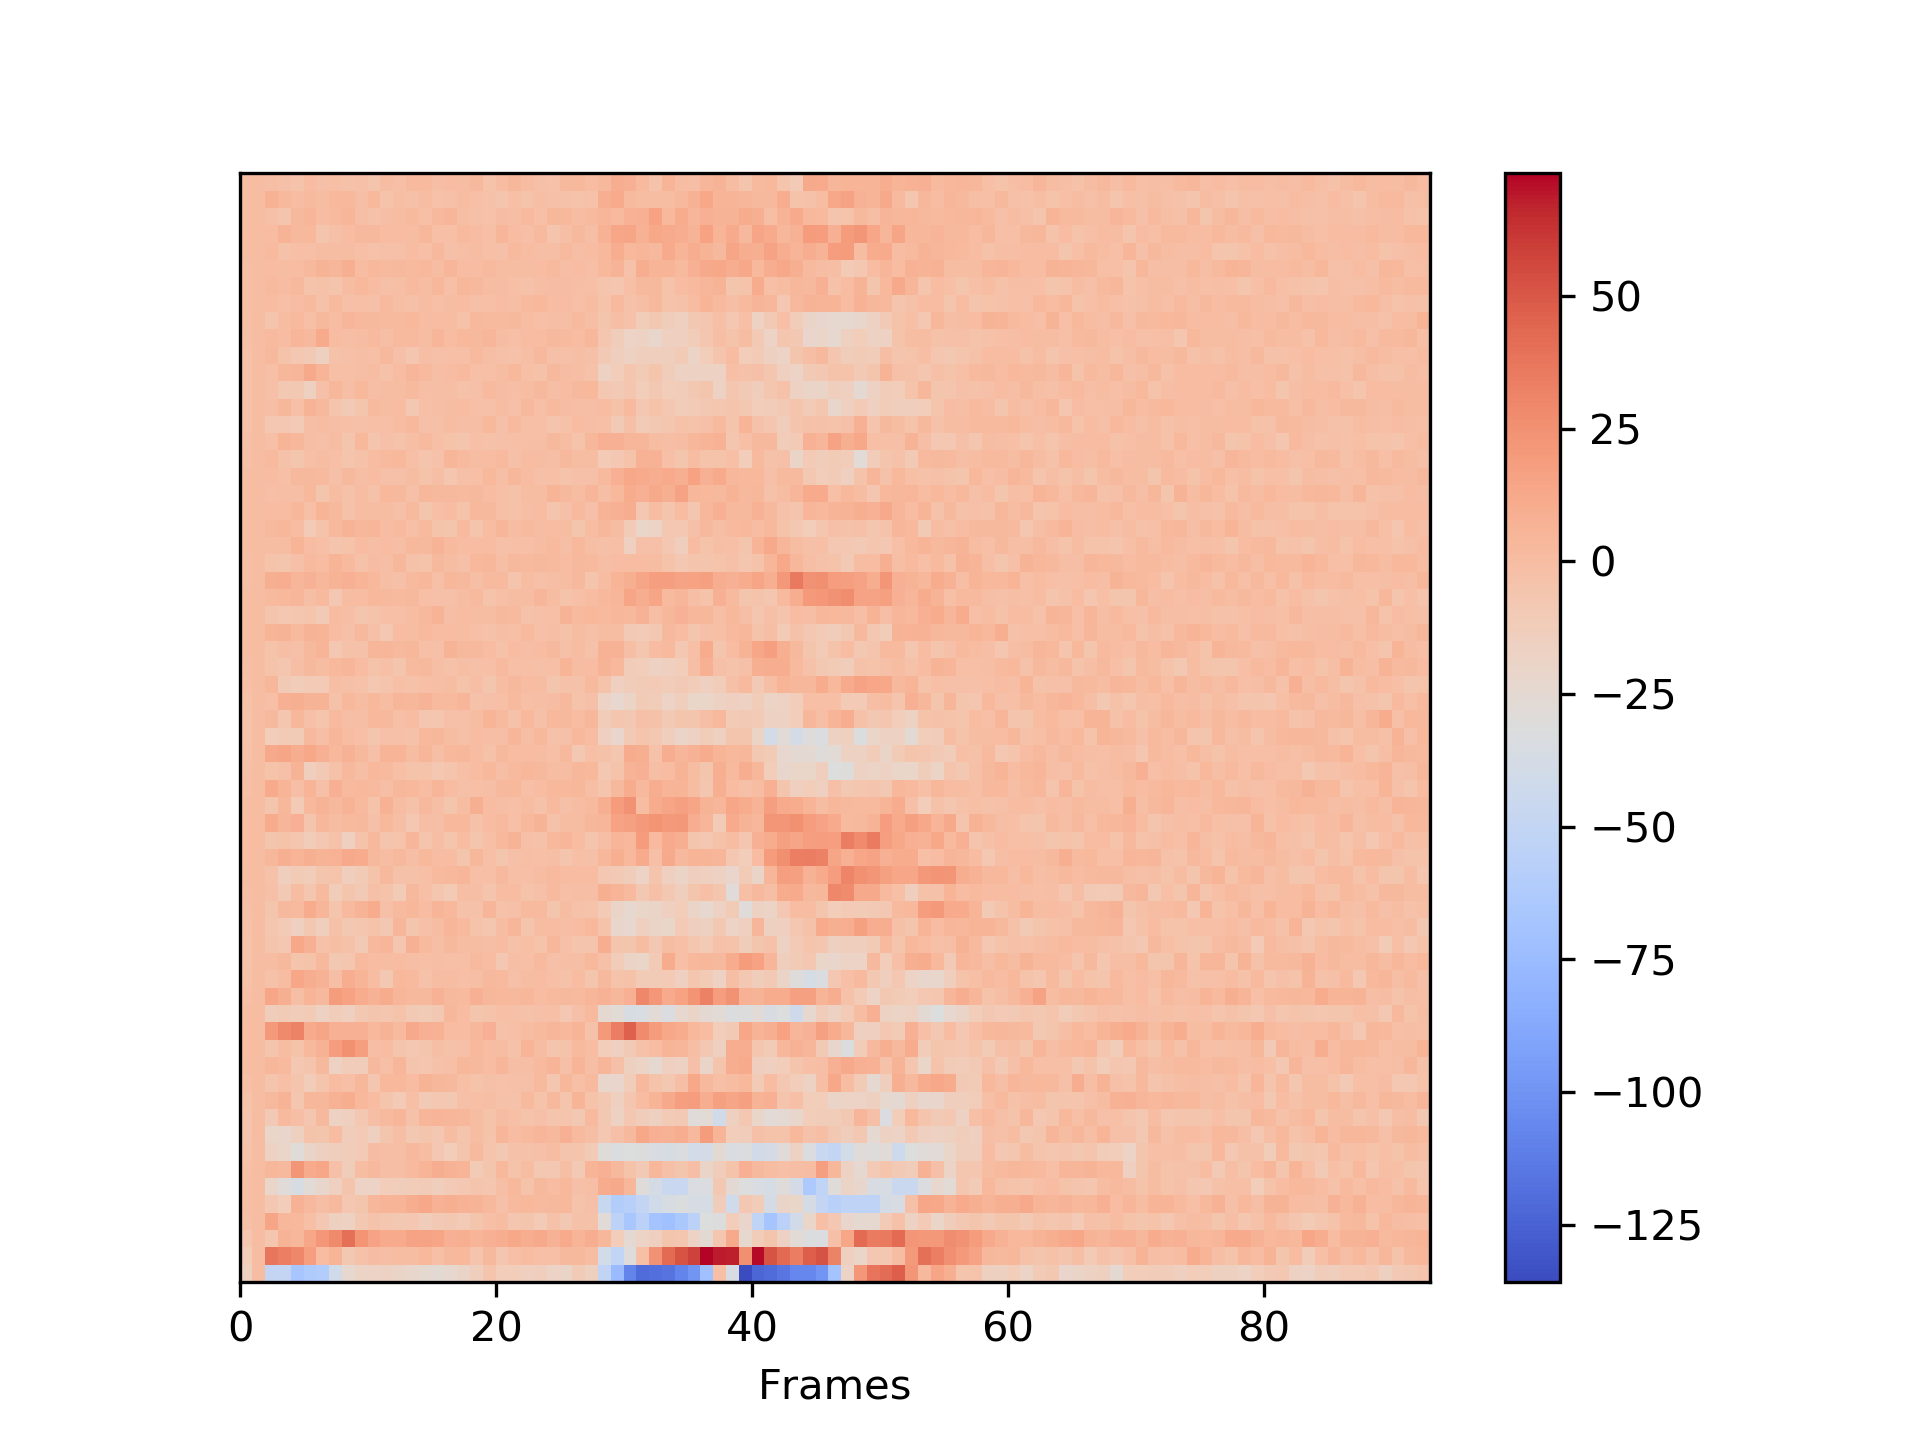
\includegraphics[width=6cm]{beijingc.png}
\caption{“北京”的MFCC系数}
\label{fig:bj}
\end{minipage}
\begin{minipage}[t]{0.48\textwidth}
\centering
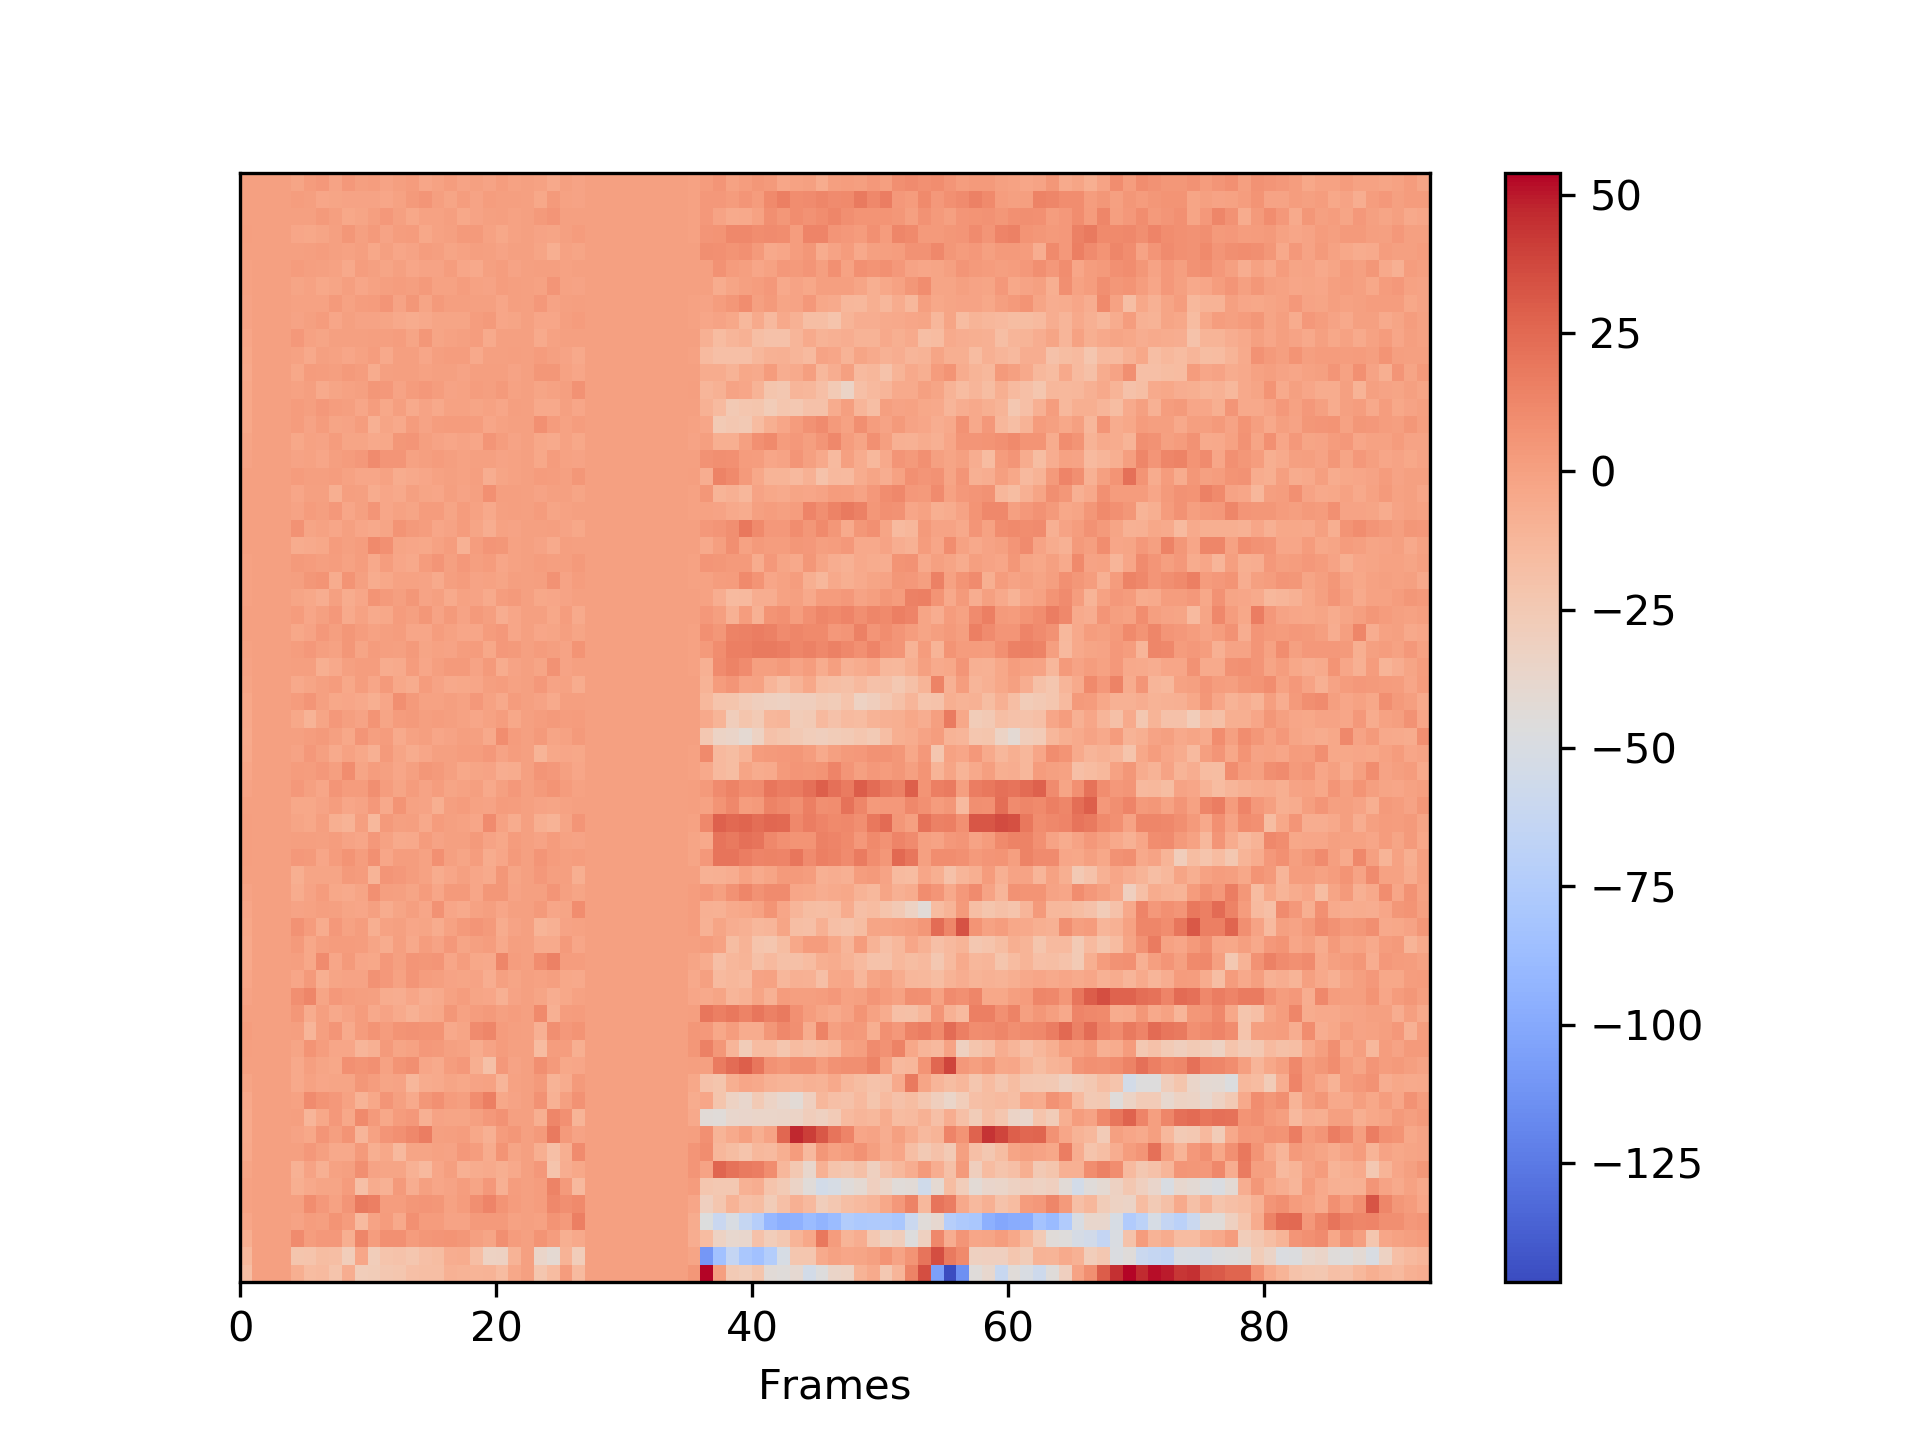
\includegraphics[width=6cm]{beijing.png}
\caption{“Beijing”的MFCC系数}
\label{fig:bjc}
\end{minipage}
\end{figure}


\section{模型}
循环神经网络(Recurrent Neural Network, RNN)和卷积神经网络(Convolutional Neural Network, CNN)是深度学习中两个比较常见的模型,其中RNN擅长表征序列信息,常用于自然语言处理,而卷积神经网络则常用于图像处理。鉴于此任务是孤立词识别,序列信息在这里面并不稳定,即语音帧之间的间隔可能会同语速有关,于是选用了CNN来作为我模型的基础架构。


\subsection{卷积神经网络}
卷积神经网络是一种常用于图像识别的神经网络模型,在语音识别上,我们可以将得到的MFCC系数当成一个图像,然后视作一个图像识别的任务即可。模型选取上,我仿照了VGG11的整体架构,稍减少不必要的参数以提高训练速度。

具体而言,模型首先是6层卷积层(卷积核大小均为3,维度分别为64, 128, 2×256, 512, 128),最后是两层全连接,维度为128,最后一层输出20维向量。卷积层之间加入批归一化来加速模型训练(很有效,速度能提高一倍),在全连接层中间加入0.5的Dropout以防过拟合。每个卷积层或全连接后加入Relu作为激活函数增加层与层之间的非线性性。

实验中发现,这样缩水后的模型在本次任务中的表现能力甚至略优,我认为这是因为数据量较少,全连接过多过大易导致过拟合,而由于我们的输入已经使用了特征提取,即MFCC系数,卷积层数过深也无法提取更多的信息。

\subsection{参数}

由于\sout{没有GPU}我对于模型进行了一定程度的优化(见上一节),在CPU上也能跑得很快。为了避免过拟合,需要把学习率调大一点,这也可以加速模型训练过程。而学习率较大,也需加大相应的,具体地我使用了0.0005的学习率,batch size为64,梯度下降算法为Adam,损失函数为交叉熵。如图\ref{fig:devtest}所示,此配置下在这个任务上训练10多个epoch后,模型收敛,验证集上可以达到99\%的准确率,而在大小为6的测试集上可以达到88\%左右。如表\ref{tb:params}。


\begin{table}[ht]
\caption{机器配置和超参选取}
\label{tb:params}
\centering
\begin{tabular}{ll}
\hline
框架 & Pytorch \\ 
CPU & AMD Ryzen 5 3550H 2.1GHz\\
内存 & 16GB \\
Batch Size & 64 \\
学习率 & 0.0005\\
梯度下降算法 & Adam \\
损失函数 & 交叉熵 \\


\hline
\end{tabular} 
\end{table}

\section{实验结果及分析}
为了避免epoch的选取,我采取了早停(Early Stopping)机制,即当模型在验证集上的表现连续三个epoch未增长时,停止训练,并取之前在验证集上分数最高的那个模型最为最终模型。其中验证集是训练集中分割出来1/10的一个样本集合,用于检验模型是否过拟合。损失函数的变化情况如图\ref{fig:loss},可见模型简单,收敛得也很快,在2个epoch中验证集准确率迅速上升至90,在之后几个epoch中微调并将测试集分数逐渐提高上来。


\begin{figure}[ht]
\centering
\begin{minipage}[t]{0.48\textwidth}
\centering
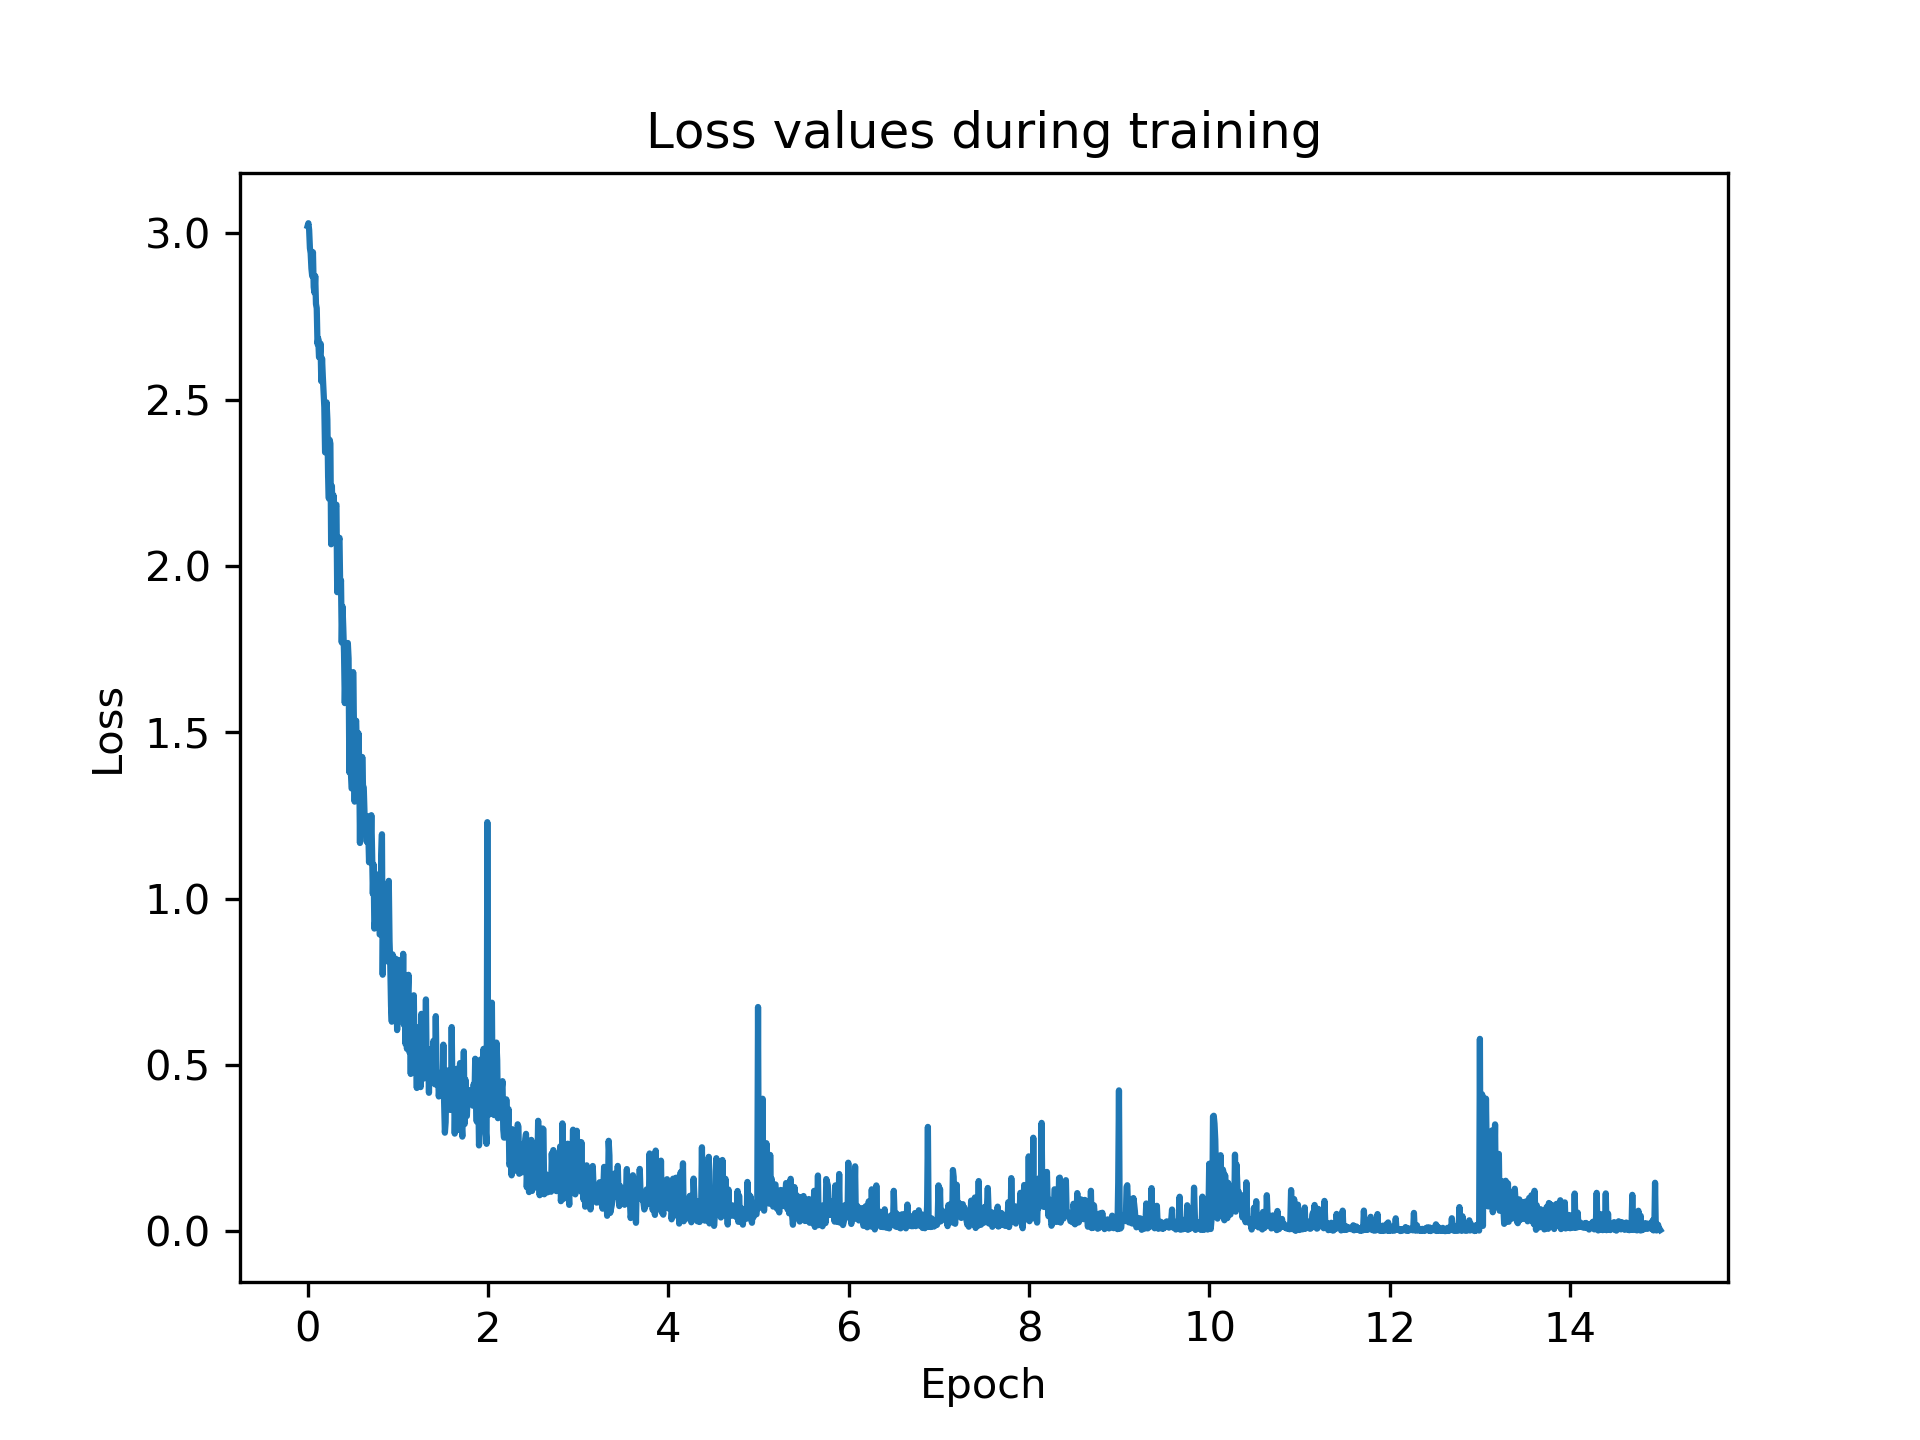
\includegraphics[width=6cm]{loss.png}
\caption{训练过程中损失函数的变化}
\label{fig:loss}
\end{minipage}
\begin{minipage}[t]{0.48\textwidth}
\centering
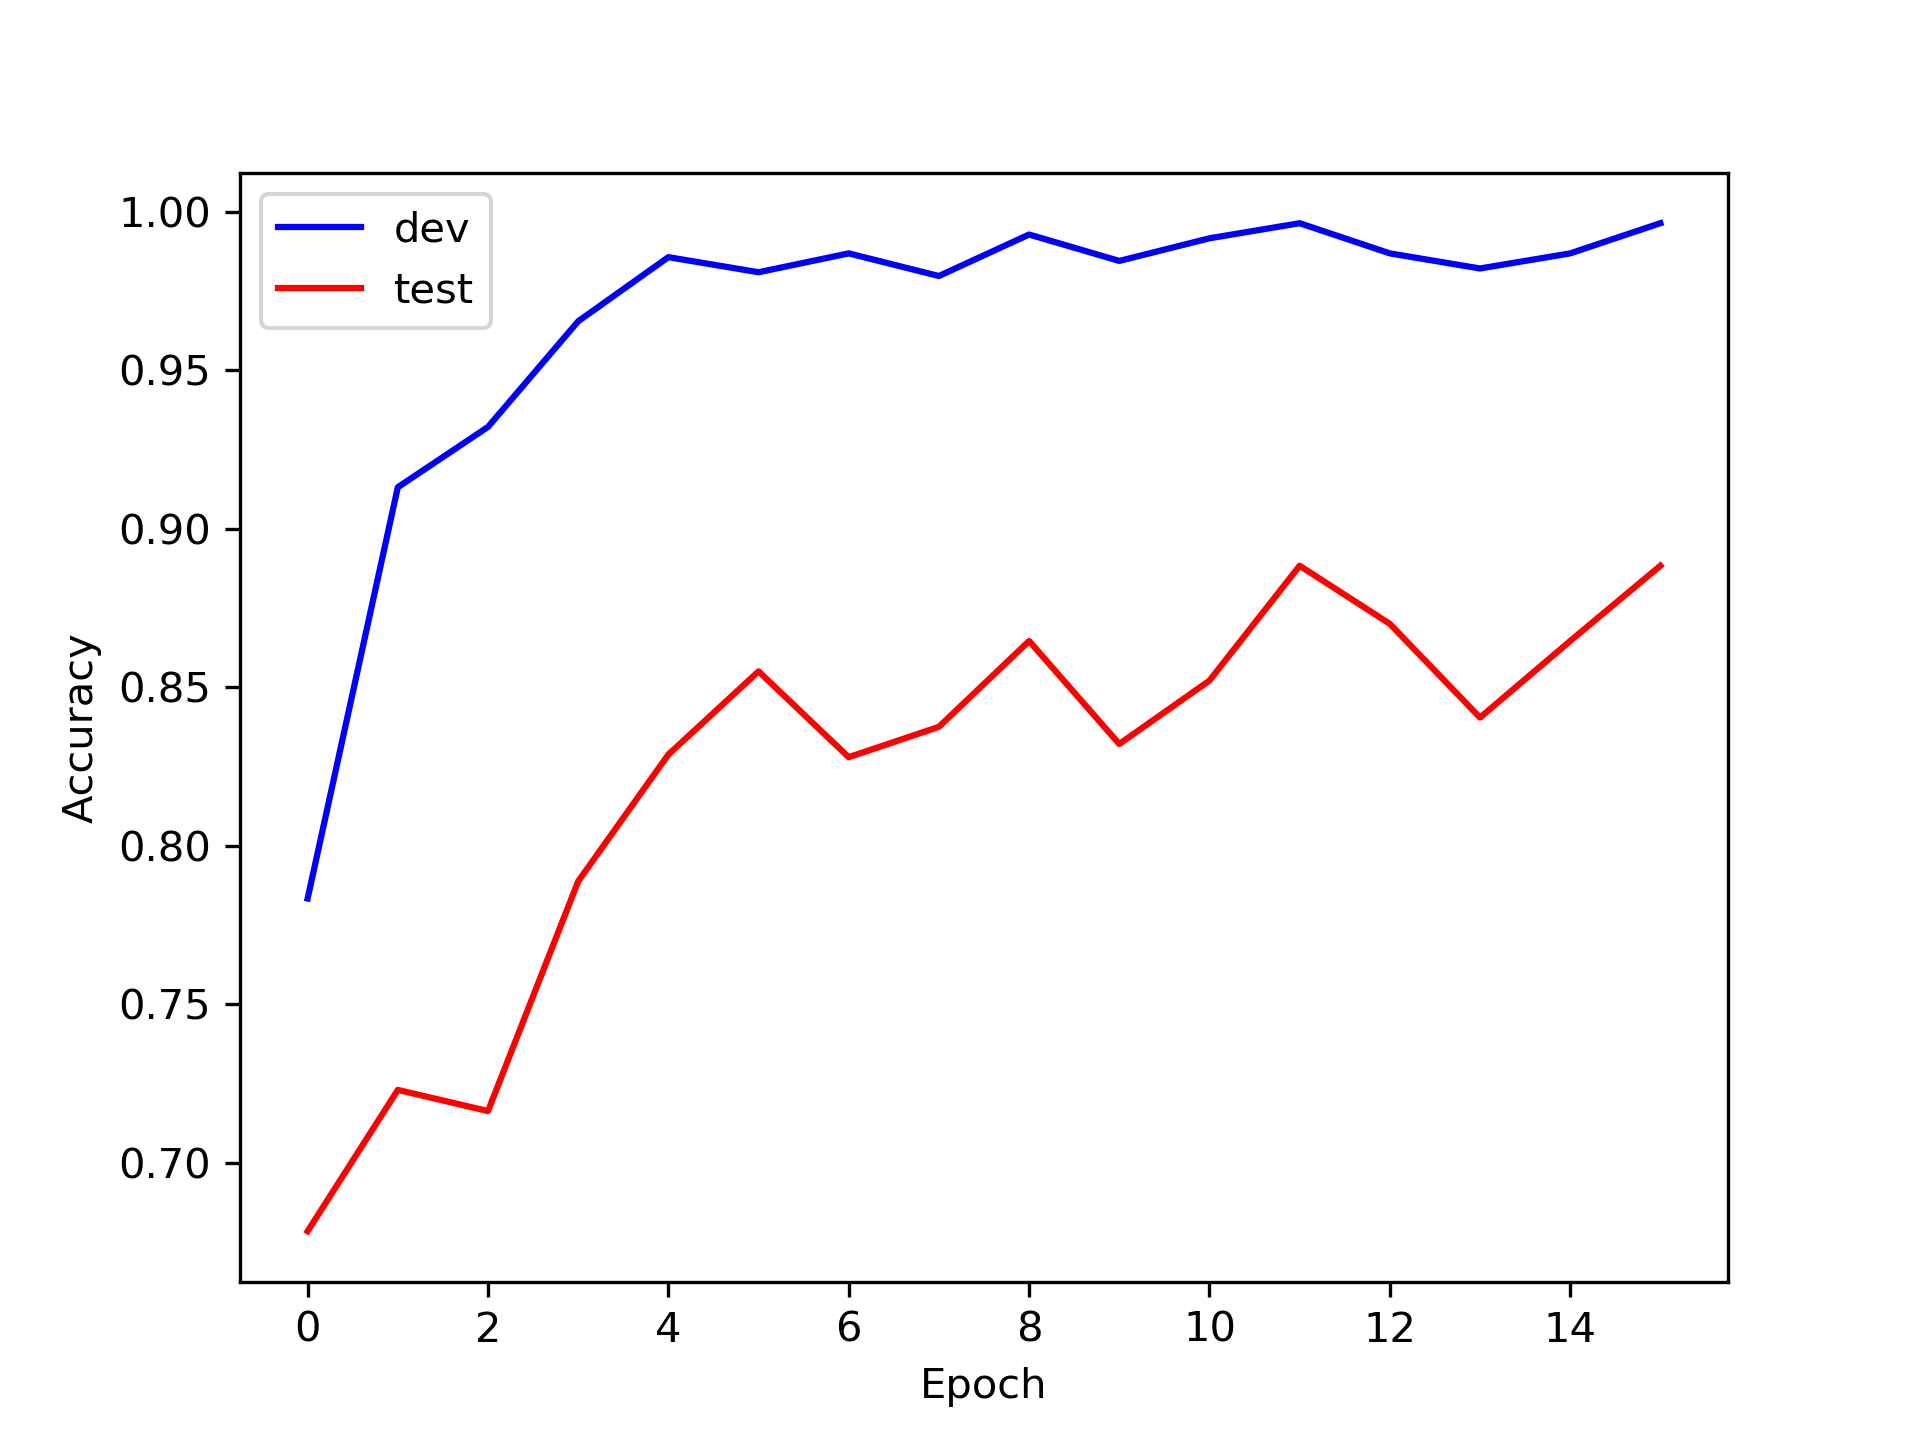
\includegraphics[width=6cm]{devtest.png}
\caption{验证集和测试集的准确率}
\label{fig:devtest}
\end{minipage}
\end{figure}

为了检验模型在各种数据大小情况下的能力,我们在测试集人数分别为6, 9, 12的情况下训练模型(按学号升序或降序排序后的前6, 9, 12个),准确率见表\ref{tb:setup},更详细的分类情况以混淆矩阵的形式在附录\ref{ch:conf}中给出。验证集由于说话人在训练集中,能达到一个很高的分数,而测试集由于不在训练集中,和验证集上的准确率相差甚远,且随着训练样本的减少而变差。其中“上海”容易被误认为是“Shanghai”、“北京”容易被误认为是“Beijing”,这也是符合直觉的。


\begin{table}[ht]
\caption{不同任务设置上的准确率}
\label{tb:setup}
\centering
\begin{tabular}{ccccc}
\hline
测试集人数 & 训练集 & 验证集 & 测试集 & 准确率(验证集/测试集) \\ 
6 & 7560 & 840 & 2400 & 99.3/88.3 \\
9 & 6480 & 720 & 3600 & 100/78.5 \\
12 & 5400 & 600 & 4800 & 99.3/67.1 \\
\hline
\end{tabular} 
\end{table}


而准确率较难上90\%的原因可能是样本中有几个容易混淆的词,且部分录音数据质量不高。而且我使用的是一维卷积,在样本数量较少的情况下表现可能并不如二维卷积,但优点在于运算速度快。


\section{总结}
在本项目中,我用一个简单而高效的基于MFCC+CNN的方法来试着完成孤立词识别任务。完整的实现了从数据预处理、特征提取、模型构建和训练的全过程,增加了我对于深度学习的应用领域——语音信号处理的基本认知和实践经验,以及对于传统特征抽取与深度学习方法的结合有了更加深入的了解。

在数据预处理时,让我意识到了数据归一化和标准化的重要性,一个合适的归一化方案可以更合理地规整数据输入以强化最终的训练效果。

在特征提取上,由于傅里叶变换比较复杂,直接用神经网络进行端到端的训练可能会比较困难,故在语音处理上,传统的特征工程仍占据一席之地。但MFCC和卷积神经网络的结合也需要相应的改变,在通常情况下,MFCC可以实现对于频域特征的压缩,阶数也通常取得较小,但事实上MFCC的阶数对于模型的表现能力还是很重要的,较大的MFCC阶数可以很好的提高模型效果。而在用语谱图和MFCC做对比实验的时候,可以发现MFCC对于语音信号的表征能力还是很不错的。

在模型方面,将语音处理转化为短时频域特征后转化为一个图像处理任务的方法,是常规且有借鉴价值的。卷积神经网络训练速度上佳,效果不至于太差,是一种很强力的深度学习模型。但可能由于我使用的是1维卷积,最后训练的效果并不是最优。


\appendix
\section{混淆矩阵表}\label{ch:conf}

\begin{table}[h]
\caption{测试集人数为6的混淆矩阵,准确率为88.3\%}
\label{tb:conf6}
\centering
\resizebox{\textwidth}{!}{
\begin{tabular}{ccccccccccccccccccccc}
\hline
  & 数字 & 语音 & 识别 & 上海 & 北京 & 考试 & 课程 & 可测 & 科创 & 客车 & Digital & Speech & Voice & Shanghai & Beijing & China & Course & Test & Coding & Code \\
 数字 & 0.983 & 0 & 0 & 0 & 0 & 0 & 0 & 0.017 & 0 & 0 & 0 & 0 & 0 & 0 & 0 & 0 & 0 & 0 & 0 & 0\\               语音 & 0 & 0.975 & 0 & 0 & 0 & 0 & 0 & 0 & 0 & 0 & 0 & 0 & 0 & 0 & 0.025 & 0 & 0 & 0 & 0 & 0\\               识别 & 0.008 & 0.008 & 0.833 & 0.017 & 0 & 0 & 0 & 0 & 0 & 0 & 0.058 & 0 & 0 & 0 & 0.008 & 0 & 0 & 0 & 0.067 & 0\\                                                                                                        上海 & 0.008 & 0 & 0 & 0.683 & 0 & 0 & 0.042 & 0 & 0.008 & 0 & 0 & 0 & 0 & 0.042 & 0 & 0 & 0.083 & 0.108 & 0 & 0.025\\                                                                                                    北京 & 0 & 0.042 & 0 & 0 & 0.758 & 0 & 0 & 0 & 0 & 0 & 0 & 0.008 & 0 & 0 & 0.192 & 0 & 0 & 0 & 0 & 0\\       考试 & 0.033 & 0 & 0 & 0 & 0 & 0.933 & 0 & 0 & 0 & 0 & 0 & 0 & 0 & 0 & 0 & 0 & 0.008 & 0 & 0 & 0.025\\       课程 & 0 & 0 & 0 & 0 & 0 & 0.008 & 0.833 & 0 & 0.05 & 0.025 & 0 & 0 & 0 & 0 & 0 & 0 & 0.017 & 0 & 0.025 & 0.042\\                                                                                                         可测 & 0.017 & 0 & 0 & 0 & 0 & 0 & 0.025 & 0.717 & 0.1 & 0.033 & 0.008 & 0 & 0 & 0 & 0.033 & 0 & 0 & 0 & 0 & 0.067\\                                                                                                      科创 & 0 & 0 & 0 & 0 & 0 & 0 & 0.008 & 0 & 0.958 & 0 & 0 & 0 & 0 & 0.008 & 0 & 0 & 0 & 0 & 0 & 0.025\\       客车 & 0 & 0 & 0 & 0 & 0 & 0 & 0.142 & 0 & 0.008 & 0.85 & 0 & 0 & 0 & 0 & 0 & 0 & 0 & 0 & 0 & 0\\            Digital & 0 & 0 & 0 & 0 & 0 & 0 & 0 & 0 & 0 & 0 & 0.917 & 0 & 0 & 0.008 & 0.008 & 0 & 0.067 & 0 & 0 & 0\\    Speech & 0 & 0 & 0 & 0 & 0 & 0 & 0 & 0 & 0 & 0 & 0 & 0.925 & 0 & 0 & 0 & 0 & 0.075 & 0 & 0 & 0\\             Voice & 0 & 0 & 0 & 0 & 0 & 0 & 0 & 0 & 0 & 0 & 0 & 0 & 0.867 & 0 & 0 & 0 & 0.125 & 0.008 & 0 & 0\\          Shanghai & 0 & 0 & 0 & 0.15 & 0 & 0 & 0 & 0 & 0 & 0 & 0 & 0 & 0 & 0.775 & 0 & 0 & 0.075 & 0 & 0 & 0\\        Beijing & 0.008 & 0 & 0 & 0 & 0.008 & 0 & 0 & 0.008 & 0 & 0 & 0 & 0 & 0 & 0 & 0.967 & 0 & 0.008 & 0 & 0 & 0\\China & 0.008 & 0.008 & 0 & 0.033 & 0 & 0 & 0 & 0 & 0 & 0 & 0 & 0 & 0 & 0 & 0 & 0.942 & 0.008 & 0 & 0 & 0\\  Course & 0 & 0 & 0 & 0.008 & 0 & 0 & 0 & 0 & 0 & 0 & 0 & 0 & 0 & 0 & 0 & 0 & 0.925 & 0.067 & 0 & 0\\         Test & 0 & 0 & 0 & 0 & 0 & 0 & 0 & 0 & 0 & 0 & 0 & 0 & 0 & 0 & 0 & 0 & 0.008 & 0.992 & 0 & 0\\               Coding & 0 & 0.008 & 0 & 0 & 0 & 0 & 0 & 0 & 0 & 0 & 0 & 0 & 0 & 0 & 0 & 0 & 0 & 0 & 0.95 & 0.042\\          Code & 0 & 0 & 0 & 0 & 0 & 0 & 0 & 0 & 0 & 0 & 0 & 0 & 0.025 & 0 & 0 & 0 & 0.075 & 0 & 0.017 & 0.883\\ 

\hline
\end{tabular}}
\end{table}

\begin{table}[ht]
\caption{测试集人数为9的混淆矩阵,准确率为78.5\%}
\label{tb:conf9}
\centering
\resizebox{\textwidth}{!}{
\begin{tabular}{ccccccccccccccccccccc}
\hline
  & 数字 & 语音 & 识别 & 上海 & 北京 & 考试 & 课程 & 可测 & 科创 & 客车 & Digital & Speech & Voice & Shanghai & Beijing & China & Course & Test & Coding & Code \\                                                        数字 & 0.928 & 0 & 0.011 & 0.056 & 0 & 0 & 0 & 0.006 & 0 & 0 & 0 & 0 & 0 & 0 & 0 & 0 & 0 & 0 & 0 & 0\\       语音 & 0 & 0.789 & 0.117 & 0 & 0.011 & 0 & 0 & 0 & 0 & 0 & 0.033 & 0 & 0 & 0 & 0.044 & 0 & 0 & 0.006 & 0 & 0\\                                                                                                            识别 & 0 & 0 & 1 & 0 & 0 & 0 & 0 & 0 & 0 & 0 & 0 & 0 & 0 & 0 & 0 & 0 & 0 & 0 & 0 & 0\\                       上海 & 0 & 0 & 0 & 0.778 & 0 & 0 & 0 & 0 & 0.006 & 0 & 0 & 0 & 0.011 & 0.2 & 0 & 0 & 0.006 & 0 & 0 & 0\\     北京 & 0.006 & 0.033 & 0 & 0 & 0.639 & 0 & 0 & 0.006 & 0 & 0.011 & 0 & 0.139 & 0 & 0 & 0.089 & 0.006 & 0 & 0.072 & 0 & 0\\                                                                                                考试 & 0.044 & 0 & 0 & 0.083 & 0 & 0.867 & 0 & 0 & 0 & 0 & 0 & 0 & 0 & 0 & 0 & 0 & 0 & 0.006 & 0 & 0\\       课程 & 0 & 0 & 0 & 0 & 0 & 0 & 0.628 & 0.017 & 0 & 0.2 & 0.006 & 0 & 0.061 & 0.006 & 0.011 & 0.022 & 0.006 & 0 & 0.006 & 0.039\\                                                                                          可测 & 0 & 0 & 0 & 0.006 & 0 & 0 & 0 & 0.578 & 0.044 & 0.328 & 0 & 0 & 0 & 0 & 0 & 0.006 & 0 & 0 & 0 & 0.039\\                                                                                                            科创 & 0 & 0 & 0 & 0.017 & 0 & 0.006 & 0.028 & 0 & 0.767 & 0.133 & 0 & 0 & 0 & 0.006 & 0.039 & 0 & 0.006 & 0 & 0 & 0\\                                                                                                    客车 & 0 & 0 & 0 & 0 & 0 & 0.028 & 0.011 & 0.05 & 0.006 & 0.85 & 0.006 & 0.006 & 0 & 0.011 & 0 & 0 & 0.006 & 0 & 0 & 0.028\\                                                                                              Digital & 0 & 0 & 0 & 0.006 & 0 & 0 & 0 & 0 & 0 & 0 & 0.917 & 0 & 0 & 0 & 0.061 & 0 & 0 & 0.011 & 0.006 & 0\\Speech & 0 & 0 & 0 & 0.006 & 0.011 & 0 & 0 & 0 & 0 & 0 & 0.011 & 0.917 & 0 & 0 & 0.033 & 0 & 0.006 & 0 & 0 & 0.017\\                                                                                                      Voice & 0 & 0 & 0 & 0 & 0 & 0 & 0 & 0 & 0 & 0 & 0 & 0.006 & 0.756 & 0 & 0 & 0.011 & 0.05 & 0.172 & 0 & 0.006\\                                                                                                            Shanghai & 0 & 0 & 0 & 0.283 & 0.006 & 0 & 0 & 0 & 0.006 & 0 & 0 & 0.006 & 0 & 0.617 & 0 & 0.039 & 0 & 0.044 & 0 & 0\\                                                                                                    Beijing & 0 & 0.011 & 0.006 & 0 & 0.4 & 0 & 0 & 0 & 0 & 0 & 0.017 & 0 & 0 & 0 & 0.561 & 0 & 0 & 0.006 & 0 & 0\\                                                                                                           China & 0 & 0 & 0 & 0.117 & 0 & 0 & 0 & 0.006 & 0 & 0 & 0 & 0 & 0 & 0.028 & 0 & 0.778 & 0 & 0.072 & 0 & 0\\  Course & 0 & 0 & 0 & 0 & 0 & 0 & 0 & 0 & 0 & 0 & 0 & 0.006 & 0.061 & 0 & 0 & 0 & 0.911 & 0.011 & 0 & 0.011\\ Test & 0 & 0 & 0 & 0.006 & 0 & 0 & 0 & 0 & 0 & 0 & 0 & 0.039 & 0 & 0 & 0 & 0 & 0 & 0.95 & 0 & 0.006\\        Coding & 0.006 & 0.017 & 0 & 0 & 0.011 & 0.039 & 0 & 0 & 0 & 0 & 0 & 0 & 0 & 0 & 0.022 & 0 & 0 & 0 & 0.828 & 0.078\\                                                                                                      Code & 0.006 & 0 & 0.006 & 0 & 0 & 0.006 & 0.033 & 0.022 & 0.022 & 0.044 & 0.017 & 0 & 0 & 0 & 0 & 0 & 0.067 & 0 & 0.128 & 0.65\\ 
\hline
\end{tabular}}
\end{table}

\begin{table}[ht]
\caption{测试集人数为12的混淆矩阵,准确率67.1\%}
\label{tb:conf12}
\centering
\resizebox{\textwidth}{!}{
\begin{tabular}{ccccccccccccccccccccc}
\hline
  & 数字 & 语音 & 识别 & 上海 & 北京 & 考试 & 课程 & 可测 & 科创 & 客车 & Digital & Speech & Voice & Shanghai & Beijing & China & Course & Test & Coding & Code \\                                                        数字 & 0.8 & 0 & 0 & 0 & 0 & 0.087 & 0 & 0.083 & 0 & 0 & 0.004 & 0 & 0.021 & 0 & 0 & 0 & 0 & 0 & 0 & 0.004\\ 语音 & 0.004 & 0.758 & 0.025 & 0 & 0.017 & 0 & 0 & 0 & 0 & 0.004 & 0.033 & 0.087 & 0.013 & 0.008 & 0.05 & 0 & 0 & 0 & 0 & 0\\                                                                                             识别 & 0.017 & 0.017 & 0.787 & 0 & 0.013 & 0.013 & 0.004 & 0.062 & 0 & 0.004 & 0 & 0.067 & 0 & 0 & 0.004 & 0.004 & 0 & 0 & 0.008 & 0\\                                                                                    上海 & 0 & 0 & 0.075 & 0.717 & 0 & 0.008 & 0 & 0.017 & 0.067 & 0 & 0 & 0.004 & 0.004 & 0.071 & 0 & 0.013 & 0.021 & 0 & 0 & 0.004\\                                                                                        北京 & 0.013 & 0 & 0 & 0 & 0.642 & 0.004 & 0 & 0.037 & 0.058 & 0 & 0.042 & 0.067 & 0 & 0 & 0.113 & 0 & 0.025 & 0 & 0 & 0\\                                                                                                考试 & 0.004 & 0 & 0 & 0 & 0 & 0.833 & 0 & 0.046 & 0.087 & 0 & 0 & 0.004 & 0.004 & 0 & 0 & 0 & 0 & 0 & 0.008 & 0.013\\                                                                                                    课程 & 0 & 0 & 0.008 & 0 & 0 & 0.05 & 0.338 & 0.292 & 0.096 & 0.037 & 0 & 0.075 & 0 & 0 & 0 & 0 & 0.008 & 0 & 0.017 & 0.079\\                                                                                             可测 & 0.008 & 0 & 0 & 0 & 0 & 0.042 & 0.021 & 0.738 & 0.008 & 0.075 & 0 & 0.083 & 0 & 0 & 0 & 0 & 0 & 0 & 0 & 0.025\\                                                                                                    科创 & 0 & 0 & 0 & 0.083 & 0 & 0 & 0.004 & 0.017 & 0.875 & 0 & 0 & 0 & 0 & 0 & 0 & 0 & 0 & 0 & 0 & 0.021\\   客车 & 0 & 0 & 0 & 0 & 0 & 0.042 & 0.004 & 0.287 & 0.104 & 0.487 & 0 & 0 & 0 & 0.046 & 0 & 0 & 0 & 0 & 0 & 0.029\\                                                                                                        Digital & 0 & 0 & 0.042 & 0.008 & 0 & 0.021 & 0 & 0.017 & 0.029 & 0 & 0.767 & 0.017 & 0.021 & 0.033 & 0 & 0.004 & 0.025 & 0 & 0 & 0.017\\                                                                                 Speech & 0 & 0 & 0.033 & 0 & 0.017 & 0.033 & 0 & 0 & 0.013 & 0 & 0.037 & 0.812 & 0.008 & 0.008 & 0 & 0.008 & 0 & 0.029 & 0 & 0\\                                                                                          Voice & 0 & 0 & 0 & 0 & 0 & 0.004 & 0 & 0.058 & 0 & 0 & 0.008 & 0.083 & 0.725 & 0.021 & 0 & 0 & 0.075 & 0.025 & 0 & 0\\                                                                                                   Shanghai & 0.025 & 0 & 0 & 0.333 & 0 & 0 & 0.05 & 0.017 & 0.067 & 0 & 0.021 & 0 & 0 & 0.45 & 0 & 0.033 & 0 & 0.004 & 0 & 0\\                                                                                              Beijing & 0 & 0 & 0 & 0 & 0.404 & 0.017 & 0.008 & 0.033 & 0.104 & 0.013 & 0.042 & 0.087 & 0 & 0 & 0.292 & 0 & 0 & 0 & 0 & 0\\                                                                                             China & 0 & 0 & 0 & 0.037 & 0 & 0.013 & 0.033 & 0.058 & 0.033 & 0 & 0 & 0.008 & 0.004 & 0.037 & 0 & 0.675 & 0.013 & 0.058 & 0.021 & 0.008\\                                                                               Course & 0 & 0 & 0 & 0 & 0 & 0.004 & 0 & 0 & 0.025 & 0 & 0.021 & 0.021 & 0 & 0 & 0 & 0 & 0.717 & 0.133 & 0 & 0.079\\                                                                                                      Test & 0 & 0 & 0.004 & 0.017 & 0.075 & 0.037 & 0.021 & 0 & 0 & 0 & 0.004 & 0.004 & 0.029 & 0.05 & 0 & 0 & 0.096 & 0.654 & 0 & 0.008\\                                                                                     Coding & 0 & 0 & 0 & 0 & 0.054 & 0.037 & 0.004 & 0.004 & 0.067 & 0 & 0 & 0.029 & 0 & 0 & 0.021 & 0 & 0.087 & 0.004 & 0.592 & 0.1\\                                                                                        Code & 0 & 0 & 0 & 0 & 0.008 & 0.071 & 0 & 0.092 & 0 & 0 & 0 & 0 & 0 & 0.004 & 0 & 0 & 0.021 & 0.033 & 0 & 0.771\\ 

\hline
\end{tabular}}
\end{table}

%\newpage
%\begin{thebibliography}{9}
%\addcontentsline{toc}{section}{参考文献}  % 目录中加入参考文献
%\bibitem{cao17}
%  Rongmei Cao.
%  Matrix Theory.
%  Nanjing University of Aeronautics and Astronautics, 2017.  

%\bibitem{pbrs14}
%  Perozzi, Bryan, R. Al-Rfou, and S. Skiena. "DeepWalk: online learning of social representations." (2014):701-710.

%\bibitem{czw17}
%  李彦冬, 郝宗波, and 雷航. "卷积神经网络研究综述." 计算机应用 36.9(2016):2508-2515.

%\end{thebibliography}

\end{document}
